%%%%%%%%%%%%%%%%%%%%%%%%%%%%%%%%%%%%%%%%%%%%%%%%%%%%%%%%%%%%%%
% --> INTRODUCCIÓN
%%%%%%%%%%%%%%%%%%%%%%%%%%%%%%%%%%%%%%%%%%%%%%%%%%%%%%%%%%%%%%
\section{Introducción}

Según \cite{R1} la programación genérica está mucho más centrada en los algoritmos que en los datos, y su postulado fundamental puede sintetizarse en una palabra: generalización. Significa que, en la medida de lo posible, los algoritmos deben ser parametrizados al máximo y expresados de la forma más independiente posible de detalles concretos, permitiendo así que puedan servir para la mayor variedad posible de tipos y estructuras de datos.

%%%%%%%%%%%%%%%%%%%%%%%%%%%%%%%%%%%%%%%%%%%%%%%%%%%%%%%%%%%%%%
% --> OBJETIVOS
%%%%%%%%%%%%%%%%%%%%%%%%%%%%%%%%%%%%%%%%%%%%%%%%%%%%%%%%%%%%%%
\subsection{Objetivos}

A continuación, se enlistan los objetivos de este laboratorio.

%%%%%%%%%%%%%%%%%%%%%%%%%%%%%%%%%%%%%%%%%%%%%%%%%%%%%%%%%%%%%%
% --> OBJETIVO GENERAL
%%%%%%%%%%%%%%%%%%%%%%%%%%%%%%%%%%%%%%%%%%%%%%%%%%%%%%%%%%%%%%
\subsubsection{Objetivo General}
\begin{itemize}
\item Diseñar una serie de clases con plantillas que permitan hacer operaciones básicas con enteros. reales, fracciones, polinomios y matrices.
\end{itemize}

%%%%%%%%%%%%%%%%%%%%%%%%%%%%%%%%%%%%%%%%%%%%%%%%%%%%%%%%%%%%%%
% --> OBJETIVOS ESPECÍFICOS
%%%%%%%%%%%%%%%%%%%%%%%%%%%%%%%%%%%%%%%%%%%%%%%%%%%%%%%%%%%%%%
\subsubsection{Objetivos Específicos}
\begin{itemize}
\item 
\item 
\item 
\end{itemize}

%%%%%%%%%%%%%%%%%%%%%%%%%%%%%%%%%%%%%%%%%%%%%%%%%%%%%%%%%%%%%%
% --> ENUNCIADO
%%%%%%%%%%%%%%%%%%%%%%%%%%%%%%%%%%%%%%%%%%%%%%%%%%%%%%%%%%%%%%
\newpage

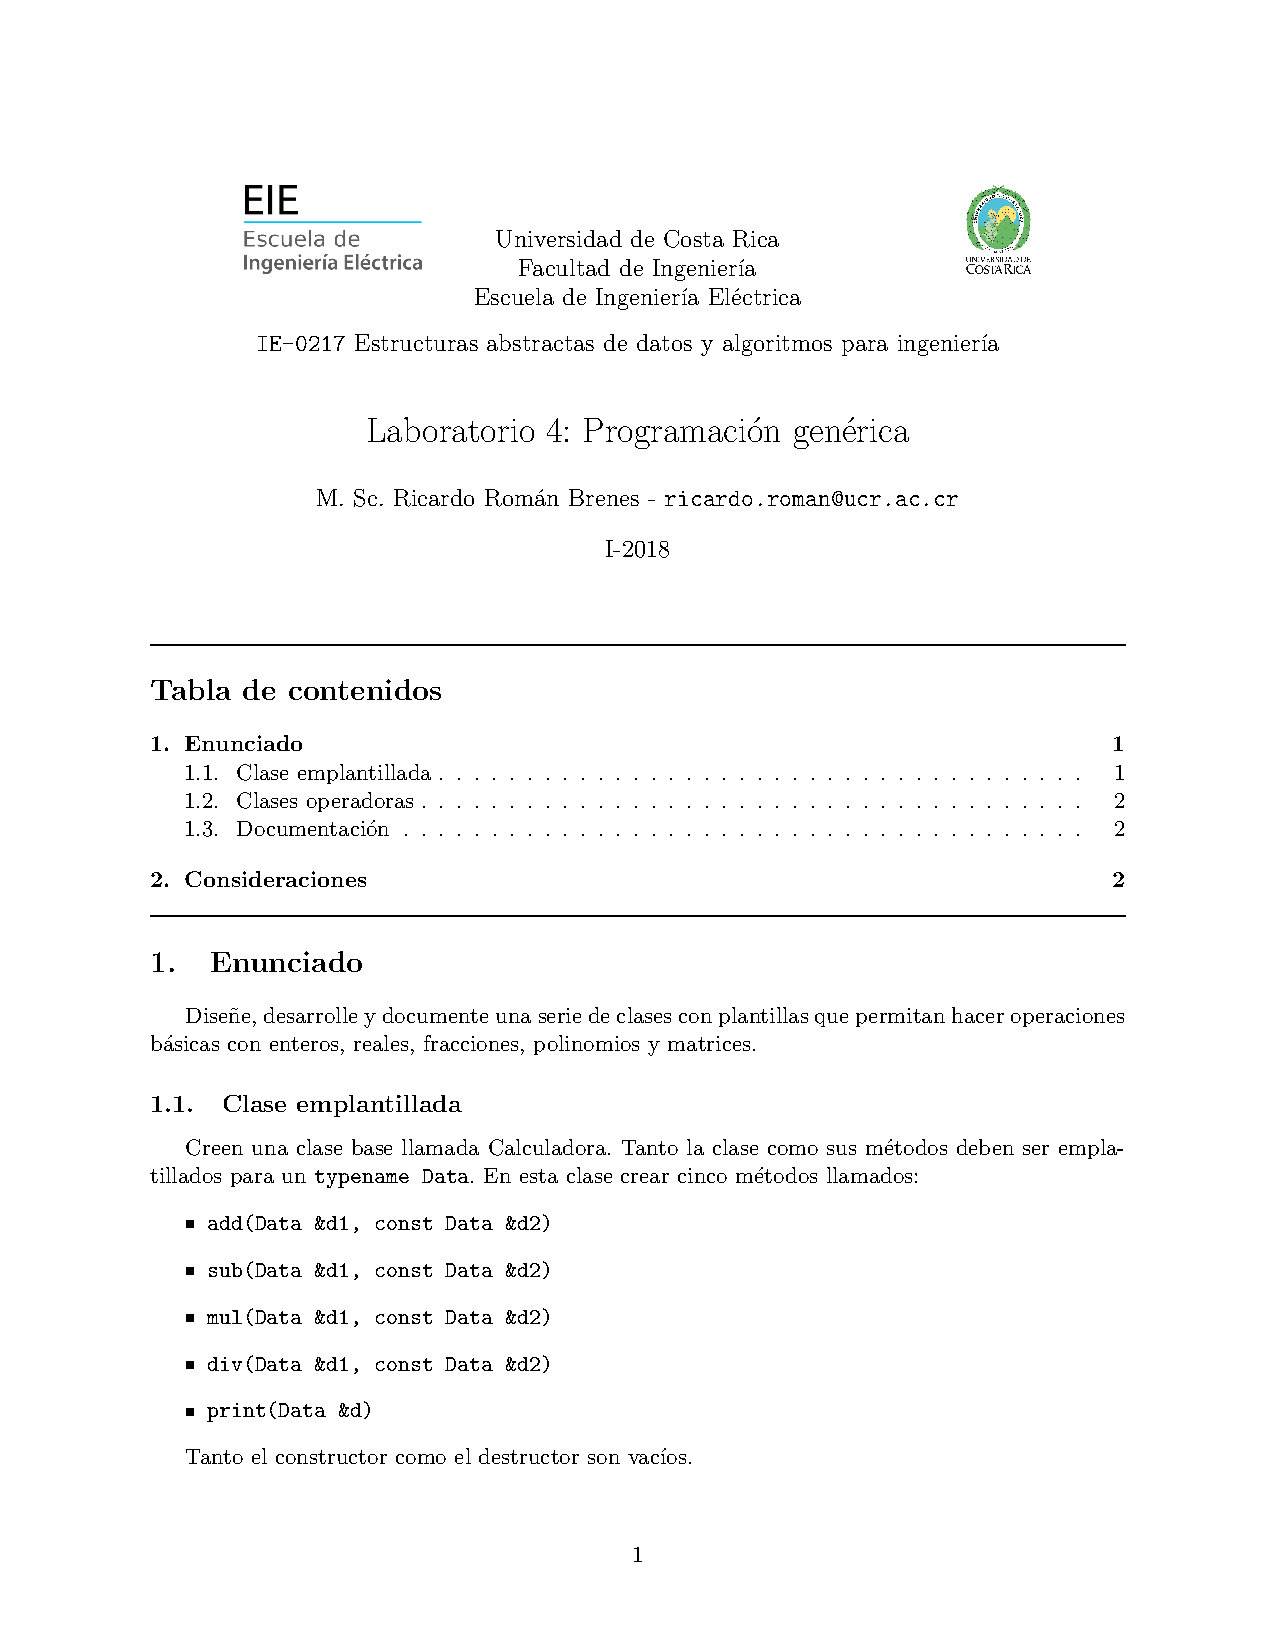
\includepdf[pages=1,pagecommand=\section{Enunciado}, scale=0.8]{enunciados/enun4} 
\includepdf[pages=2,pagecommand={},scale=0.8]{enunciados/enun4}

%%%%%%%%%%%%%%%%%%%%%%%%%%%%%%%%%%%%%%%%%%%%%%%%%%%%%%%%%%%%%%
% --> SOLUCIÓN
%%%%%%%%%%%%%%%%%%%%%%%%%%%%%%%%%%%%%%%%%%%%%%%%%%%%%%%%%%%%%%
\section{Solución}

%%%%%%%%%%%%%%%%%%%%%%%%%%%%%%%%%%%%%%%%%%%%%%%%%%%%%%%%%%%%%%
% --> CLASE POLINOMIO
%%%%%%%%%%%%%%%%%%%%%%%%%%%%%%%%%%%%%%%%%%%%%%%%%%%%%%%%%%%%%%
\subsection{Clase Polinomio}

La clase \texttt{Polynomial} realiza operaciones básicas de polinomios de grado n. En este archivo \texttt{.h} se declaran todas las funciones necesarias, así como dos variables necesarias para la ejecución, una tipo \texttt{int} para almacenar el tamaño del polinomio, es decir, la cantidad de coeficientes que posee. Y otra variable tipo \texttt{double*} para almacenar estos coeficientes, esto es un puntero que básicamente funciona como un \texttt{array}.

\begin{minted}[linenos,autogobble,bgcolor=bg,breaklines,fontsize=\footnotesize ]{c++}
class Polynomial
{
	public:
		Polynomial	(int Grado,double Coeficientes[]);
		Polynomial	(const Polynomial &l_cCopyPolynomial);
		~Polynomial	();
		Polynomial 	operator+(const Polynomial &P);
		Polynomial 	operator-(const Polynomial &P);
		Polynomial 	operator*(const Polynomial &P);
		Polynomial	operator/(const Polynomial &P);
		void 				operator~(void);
	protected:
		double* m_pCoefPolinomio;
	private:
		int m_iTamPolinomio;

};

\end{minted}

\subsubsection{Métodos de \texttt{Polynomial()}.}
\begin{itemize}
    \item \textbf{Método constructor:}
    
    El método constructor por defecto requiere de dos argumentos, uno es el grado del polinomio, y el otro es un arreglo del tipo \texttt{double} con los coeficientes que conforman el polinomio.  
\end{itemize}

%%%%%%%%%%%%%%%%%%%%%%%%%%%%%%%%%%%%%%%%%%%%%%%%%%%%%%%%%%%%%%
% --> CLASE FRACCIÓN
%%%%%%%%%%%%%%%%%%%%%%%%%%%%%%%%%%%%%%%%%%%%%%%%%%%%%%%%%%%%%%
\subsection{Clase Fracción}

\begin{minted}[linenos,autogobble,bgcolor=bg,breaklines,fontsize=\footnotesize ]{c++}
class Fraction
{
	public:
		Fraction();
		Fraction(int l_iNum, int l_iDen);
		Fraction(const Fraction &l_cCopyFraction);
		~Fraction();
		Fraction operator+(const Fraction &rhs);
		Fraction operator-(const Fraction &rhs);
		Fraction operator*(const Fraction &rhs);
		Fraction operator/(const Fraction &rhs);
		void operator~();
	protected:
	private:
		int m_iNumerador;
		int m_iDenominador;
		void checkDen();
};
\end{minted}


%%%%%%%%%%%%%%%%%%%%%%%%%%%%%%%%%%%%%%%%%%%%%%%%%%%%%%%%%%%%%%
% --> CLASE MATRIZ
%%%%%%%%%%%%%%%%%%%%%%%%%%%%%%%%%%%%%%%%%%%%%%%%%%%%%%%%%%%%%%
\subsection{Clase Matriz}

\begin{minted}[linenos,autogobble,bgcolor=bg,breaklines,fontsize=\footnotesize ]{c++}
class Matrix
{
	public:
		Matrix		(int l_iRowSize, int l_iColSize, bool l_bFlag);
		Matrix		(double* l_pMatrix, int l_iRowSize, int l_iColSize);
		Matrix		(const Matrix &l_cCopyMat);
		~Matrix		();
		Matrix 		operator+(const Matrix &rhs);
		Matrix 		operator-(const Matrix &rhs);
		Matrix 		operator*(const Matrix &rhs);
		Matrix 		operator/(const Matrix &rhs);
		int 			GetRowSize();
		int 			GetColsSize();
		double 		GetMatValue(int l_iRow, int l_iCol);
		void  		SetMatValue(int l_iRC, double l_dValue);
		void 			operator~(void);
	protected:
	private:
		double* 	m_pMatrix;
		int 			m_iRows;
		int 			m_iCols;
};
\end{minted}

%%%%%%%%%%%%%%%%%%%%%%%%%%%%%%%%%%%%%%%%%%%%%%%%%%%%%%%%%%%%%%
% --> CLASE CALCULADORA
%%%%%%%%%%%%%%%%%%%%%%%%%%%%%%%%%%%%%%%%%%%%%%%%%%%%%%%%%%%%%%
\subsection{Clase Calculadora}

\begin{minted}[linenos,autogobble,bgcolor=bg,breaklines,fontsize=\footnotesize ]{c++}
#ifndef CALCULATOR_H
#define CALCULATOR_H

#include <iostream>
#include <string>
#include <math.h>
#include "fraction.h"
#include "matrix.h"
#include "polynomial.h"

using namespace std;

template<typename Data>
class Calculator
{
	public:
		Calculator(){};
		~Calculator(){};
		Data add(Data &d1, const Data &d2) {return d1+d2;};
		Data sub(Data &d1, const Data &d2) {return d1-d2;};
		Data mul(Data &d1, const Data &d2) {return d1*d2;};
		Data div(Data &d1, const Data &d2) {return d1/d2;};
		void print(Data &d){~d;};
	protected:
	private:
};

#endif //CALCULATOR_H
\end{minted}

%%%%%%%%%%%%%%%%%%%%%%%%%%%%%%%%%%%%%%%%%%%%%%%%%%%%%%%%%%%%%%
% --> MAIN
%%%%%%%%%%%%%%%%%%%%%%%%%%%%%%%%%%%%%%%%%%%%%%%%%%%%%%%%%%%%%%
\subsection{Programa Principal}

\begin{minted}[linenos,autogobble,bgcolor=bg,breaklines,fontsize=\footnotesize ]{c++}
class Matrix
{
	public:
		Matrix		(int l_iRowSize, int l_iColSize, bool l_bFlag);
		Matrix		(double* l_pMatrix, int l_iRowSize, int l_iColSize);
		Matrix		(const Matrix &l_cCopyMat);
		~Matrix		();
		Matrix 		operator+(const Matrix &rhs);
		Matrix 		operator-(const Matrix &rhs);
		Matrix 		operator*(const Matrix &rhs);
		Matrix 		operator/(const Matrix &rhs);
		int 			GetRowSize();
		int 			GetColsSize();
		double 		GetMatValue(int l_iRow, int l_iCol);
		void  		SetMatValue(int l_iRC, double l_dValue);
		void 			operator~(void);
	protected:
	private:
		double* 	m_pMatrix;
		int 			m_iRows;
		int 			m_iCols;
};
\end{minted}

%%%%%%%%%%%%%%%%%%%%%%%%%%%%%%%%%%%%%%%%%%%%%%%%%%%%%%%%%%%%%%
% --> RESULTADOS
%%%%%%%%%%%%%%%%%%%%%%%%%%%%%%%%%%%%%%%%%%%%%%%%%%%%%%%%%%%%%%
\section{Resultados}


%%%%%%%%%%%%%%%%%%%%%%%%%%%%%%%%%%%%%%%%%%%%%%%%%%%%%%%%%%%%%%
% --> CONCLUSIONES
%%%%%%%%%%%%%%%%%%%%%%%%%%%%%%%%%%%%%%%%%%%%%%%%%%%%%%%%%%%%%%
\section{Conclusiones}


Como conclusiones se tiene que:

\begin{itemize}
\item fd
\end{itemize}


%%%%%%%%%%%%%%%%%%%%%%%%%%%%%%%%%%%%%%%%%%%%%%%%%%%%%%%%%%%%%%
% --> BIBLIOGRAFIA
%%%%%%%%%%%%%%%%%%%%%%%%%%%%%%%%%%%%%%%%%%%%%%%%%%%%%%%%%%%%%%
\begin{thebibliography}{IEEE}
\bibitem{R1} Talens, S. \textbf{\textit{Curso de programación en C++}}. EUI (UPV) Valencia, 17 al 28 de Julio de 1995. 
\end{thebibliography}
